\section{Lịch sử máy tính} 


Máy tính ngày nay có một phả hệ hết sức rộng rãi. Một trong những thiết bị tính toán ra
đời sớm nhất là bàn tính, được biết đến từ thời La Mã và Hy Lạp cổ đại. Máy này khá đơn
giản, bao gồm các hạt tròn được xâu lần lượt trên các que gắn trong một khung chữ nhật
(Hình \ref{fig:fig0.3}). Các hạt này có thể di chuyển qua lại trên các que, và các vị trí
của chúng thể hiện các giá trị lưu trữ. Vậy ``máy tính'' này biểu diễn và lưu trữ dữ liệu
chính trong các vị trí của các hạt này. Để điều khiển việc thực hiện thuật toán, máy phải
dựa vào người thao tác. Bởi vậy bản thân bàn tính chỉ đóng vai trò lưu trữ dữ liệu; nó
phải kết hợp với hoạt động của con người để tạo ra một máy hoàn chỉnh có thể tính toán
được.


\begin{figure}[tb]
\centering
    \scalebox{0.4}{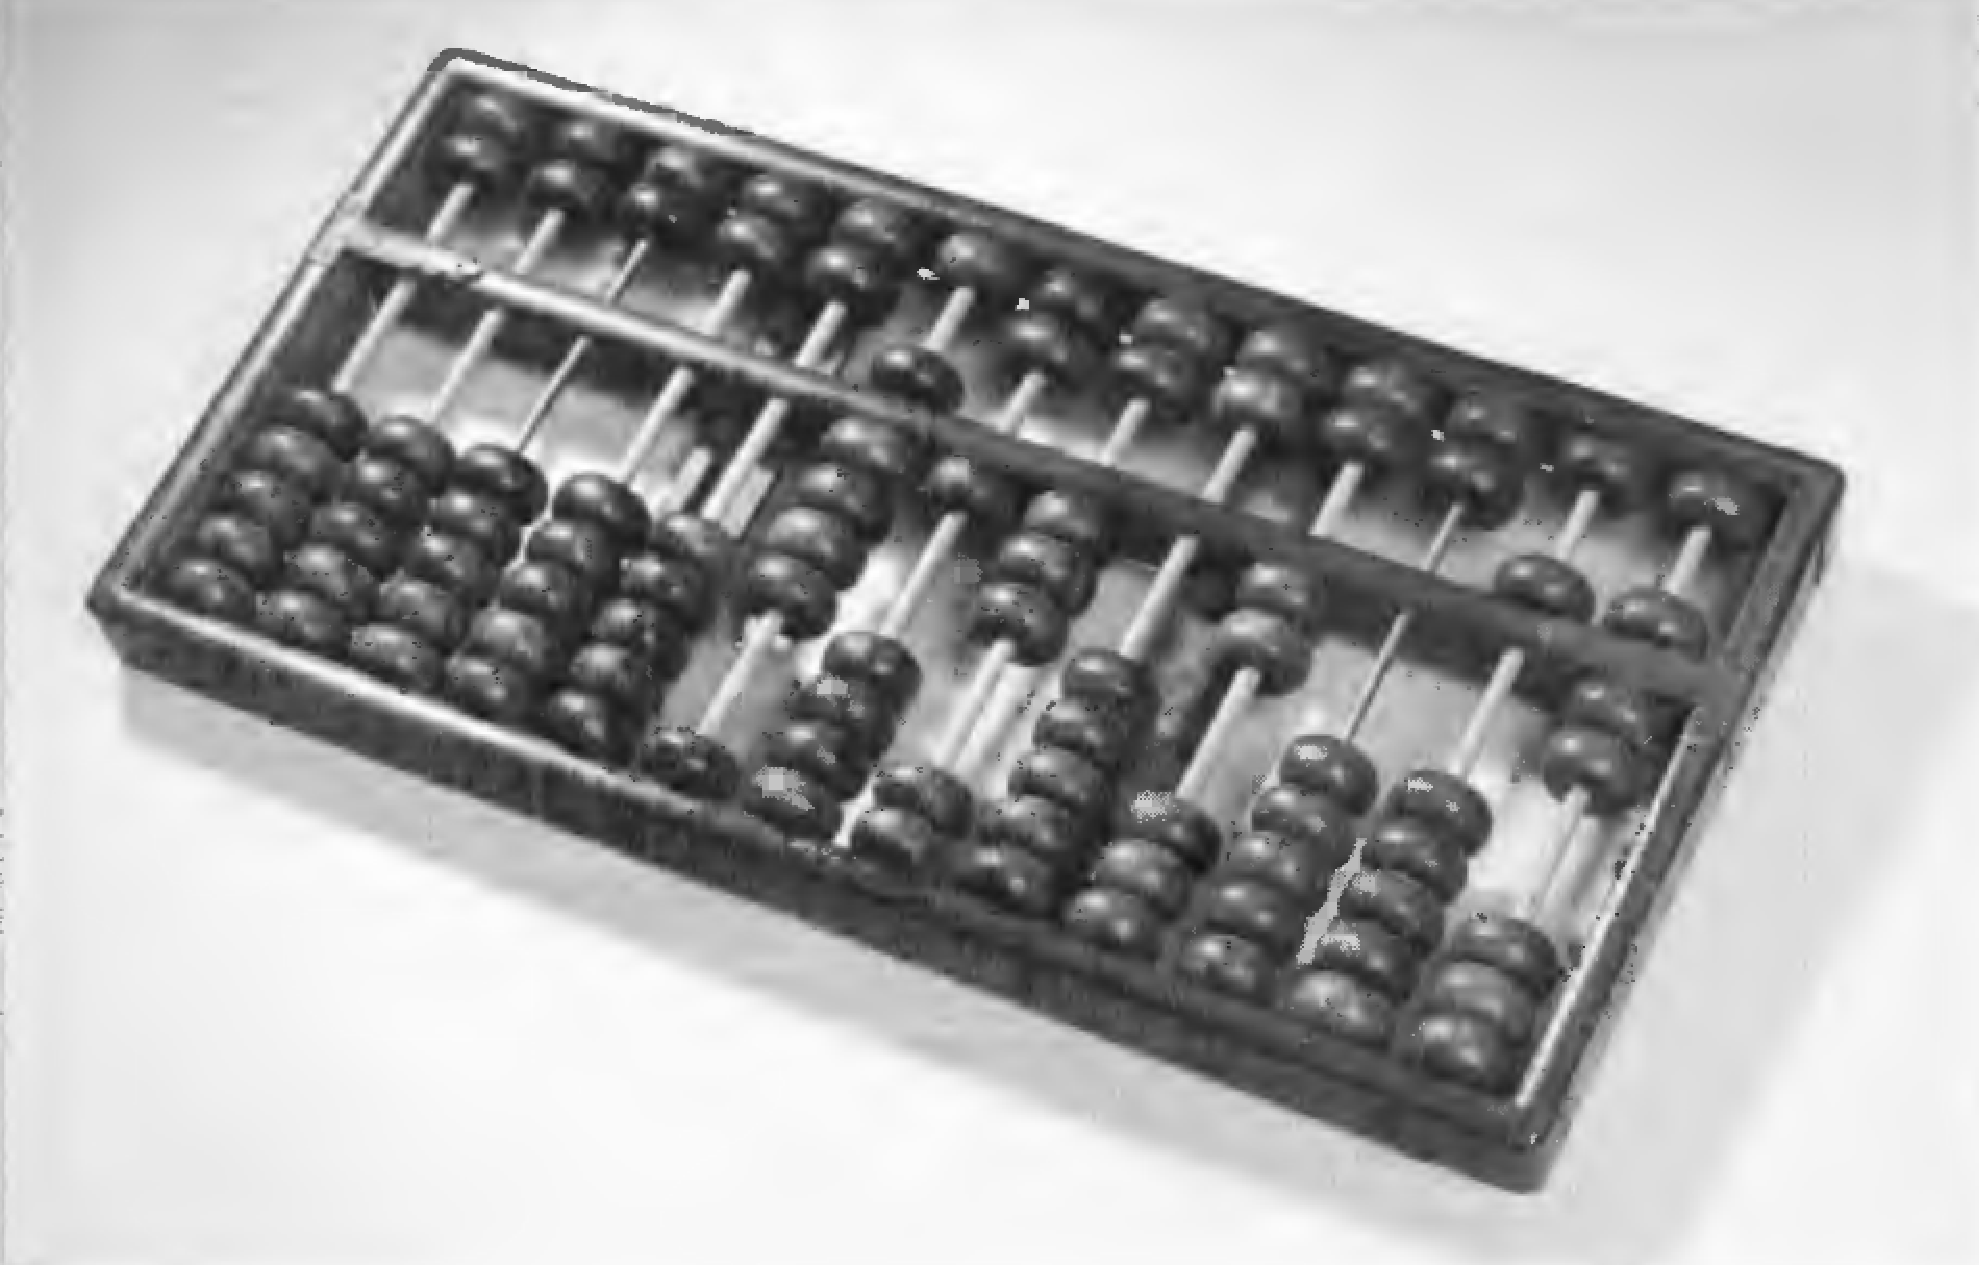
\includegraphics{ch0/fig03.pdf}}
\caption{Một bàn tính (ảnh chụp bởi Wayne Chandler)}
  \label{fig:fig0.3}
\end{figure}
 


Gần đây hơn, các thiết kế của máy tính đã dựa trên công nghệ cơ học. Một số nhà phát minh
trong thời kỳ này là Blaise Pascal (1623-1662) của Pháp, Wilhelm Gottfried Leibniz
(1646-1716) của Đức, và Charles Babbage (1792-1871) của Anh. Những máy này biểu diễn dữ
liệu thông qua vị trí của bánh răng, với các dữ liệu đầu vào được đặt một cách cơ học bằng
vị trí ban đầu của bánh răng.  Đầu ra của các máy của Pascal và của Leibniz đã được xác
định bằng cách quan sát các vị trí của bánh răng khi việc thực hiện kết thúc. Để tránh các sai sót khi ghi lại kết quả tính toán, 
Babbage đã thiết kế máy cho phép in luôn kết quả tính toán ra giấy.


Ta có thể thấy các máy ngày càng linh hoạt hơn (theo nghĩa làm việc theo thuật toán). Máy
của Pascal chỉ thực hiện phép cộng đơn giản bằng cách đặt một dãy các bước thích hợp ngay
trong bản thân cấu trúc của máy. Tương tự, máy của Leibniz có thuật toán được nhúng sẵn
vào trong kiến trúc của nó, mặc dù nó đã cho phép người dùng thao tác để lựa chọn trong
nhiều phép toán số học. Máy tính sai phân của Babbage (Babbage's Difference Engine), thực
ra nó vẫn chỉ là mô hình trên giấy, có thể thay đổi thực hiện nhiều phép toán phong phú;
và máy Phân tích (Analytical Engine), máy mà Babbage chưa bao giờ nhận được tài trợ để
làm, đã được thiết kế để đọc các lệnh dưới dạng các lỗ trên thẻ giấy. Bởi vậy máy Phân
tích của Babbage là có thể lập trình được. Trên thực tế, Augusta Ada Byron (Ada Lovelace)
đã xuất bản một bài báo chỉ ra cách lập trình trên máy Phân tích để thực hiện nhiều tính
toán. Và ngày nay người ta vẫn xem Ada như lập trình viên đầu tiên trên thế giới.


Ý tưởng biểu diễn các thuật toán thông qua giấy đục lỗ không phải bắt đầu từ Babbage. Ông
đã dựa trên ý tưởng trước đó của Joseph~Jacquard (1752-1834). Vào năm 1801,
Joseph Jacquard đã tạo nên một khung dệt, mà trong đó từng bước của quá trình dệt đã được
xác định bởi các mẫu lỗ đục trên thẻ giấy. Theo cách này, các thuật toán được thực hiện
bởi các khung dệt có thể thay đổi một cách dễ dàng theo các thiết kế mẫu dệt khác
nhau. Herman Hollerith (1860-1929) cũng đã sử dụng ý tưởng của Jacquard để tăng tốc độ xử
lý các bảng tính trong điều tra số dân của Mỹ năm 1890. Kiểu thẻ này sau đó đã được gọi là
thẻ đục lỗ đã là một phương tiện giao tiếp với máy tính rất phổ biến vào những năm
1970s. Cho đến nay các kỹ thuật này vẫn được sử dụng, như trong cuộc bầu cử tổng thống Mỹ
năm 2000.

Do hạn chế về công nghệ, việc sản xuất các máy cơ học phức tạp của của Pascal, Leibniz, và
Babbage thời đó rất tốn kém. Nhưng với những tiến bộ trong công nghệ điện tử vào đầu năm
1900, trở ngại này đã được khắc phục. Ví dụ như máy điện của George Stibitz, hoàn thành
trong 1940 tại phòng thí nghiệm Bell, và máy Mark I, hoàn thành năm 1944 tại Đại học
Harvard bởi Howard Aiken và một nhóm kỹ sư của IBM (Hình \ref{fig:fig0.4}). Nhưng các máy
này dùng các rơle cơ học điện tử, trong khi các nhà nghiên cứu khác đã áp dụng các kỹ
thuật ống chân không, nên chúng đã bị lỗi thời ngay sau khi được xây dựng. Một trong những
chiếc máy đầu tiên sử dụng công nghệ ống chân không là máy Atanasoff-Berry do John
Atanasoff và trợ lý của mình là Clifford Berry xây dựng trong thời kỳ từ 1937 đến 1941 tại
Iowa State College (nay là Đại học bang Iowa). Một máy khác được gọi là Colossus, đã được
xây dựng dưới sự chỉ đạo của Tommy Flower ở Anh để giải mã các bức điện bằng Tiếng Đức
trong Thế chiến thứ II (World War II). (Trên thực tế, người ta đã làm khoảng mười chiếc
máy. Nhưng vì lý do bí mật quân sự và an ninh quốc gia nên người ta đã không công bố, do
đó những chiếc máy này không trở thành một phần trong ``cây phả hệ của họ máy tính''.)
Sau đó, đã có các máy linh hoạt hơn, như ENIAC (Electronic Numerical Intergrator and
Calculator) được phát triển bởi John Mauchly và J. Presper Eckert tại Trường Moore thuộc
khoa Công nghệ Điện tử, Đại học Pennsylvania.

\begin{figure}[tb]
\centering
    \scalebox{0.5}{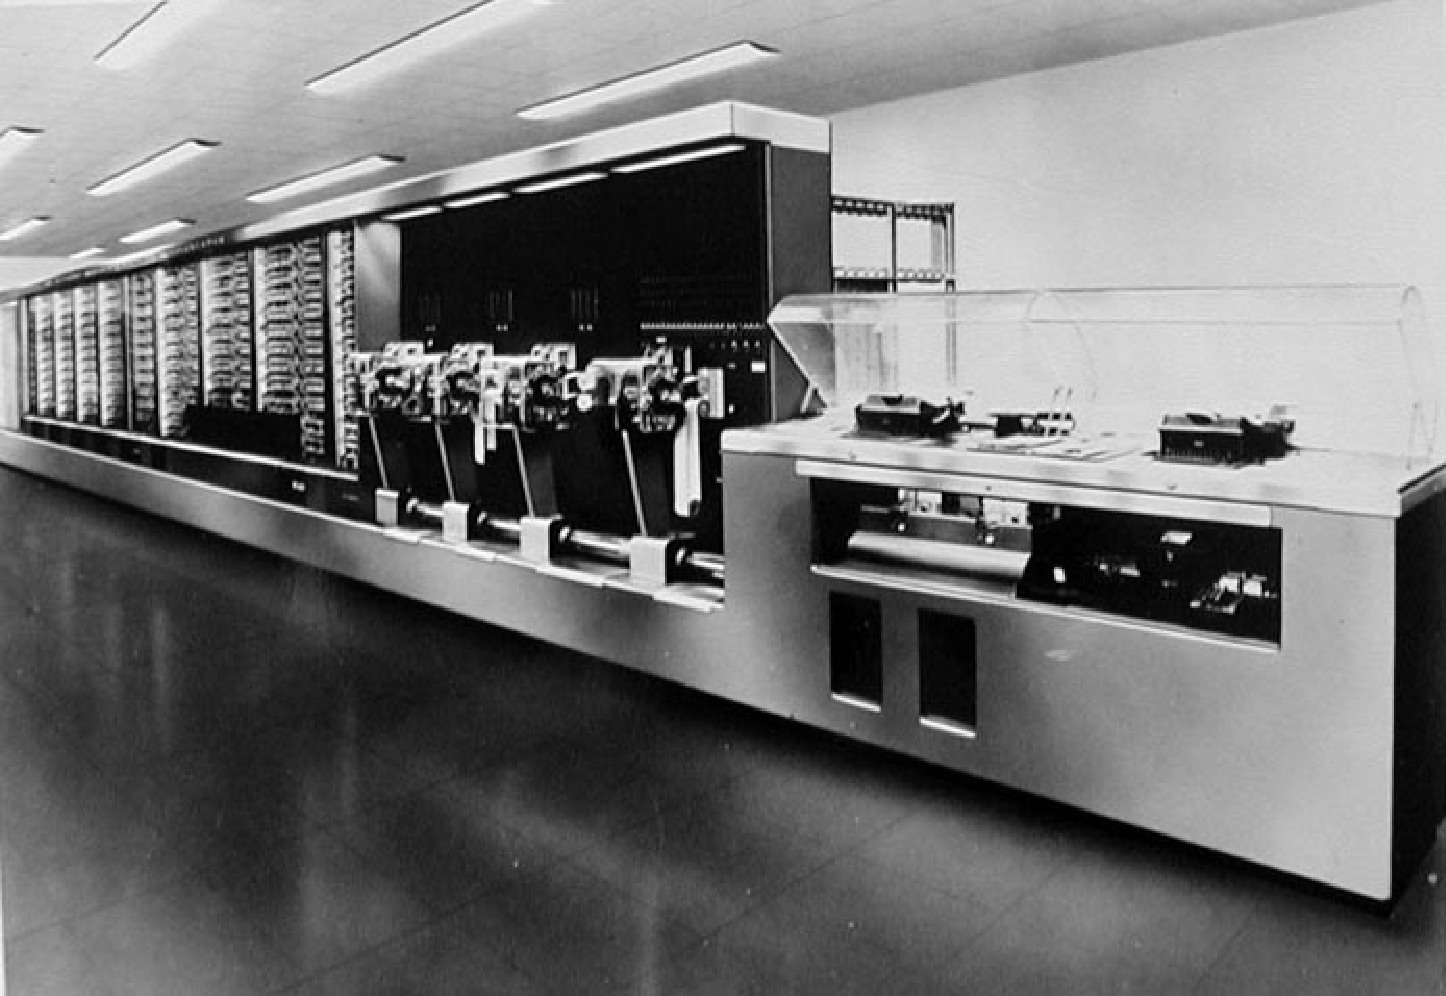
\includegraphics{ch0/fig04.pdf}}
\caption{Máy tính Mark I}
  \label{fig:fig0.4}
\end{figure}


Từ đó đến nay, lịch sử của máy tính gắn liền với việc phát triển công nghệ, bao gồm việc
phát minh ra transitors và sau đó là sự phát triển của các mạch tích hợp, sự xuất hiện
truyền thông qua vệ tinh, và tiến bộ trong công nghệ quang. Ngày nay, một chiếc máy tính
nhỏ cầm tay có thể có hiệu suất tính toán lớn hơn so với máy tính kích thước bằng cả căn
phòng của những năm 1940 và có thể trao đổi thông tin nhanh chóng qua qua hệ thống truyền
thông toàn cầu.

Một bước quan trọng làm cho máy tính trở nên phổ biến là sự phát triển của máy tính để
bàn~(desktop computer).  Những máy này bắt nguồn từ những người ưa thích máy tính, họ bắt
đầu thử tự làm các máy tính tại nhà ngay sau khi có những chiếc máy tính dùng trong nghiên
cứu vào những năm 1940. Cũng chính vì ham thích, Steve Jobs và Stephen Wozniak đã tạo ra
chiếc máy tính dùng ở nhà có thể thương mại được, và đến năm 1976, họ đã thành lập Apple
Computer, Inc, để sản xuất và bán các sản phẩm của họ. Các công ty khác cũng có các sản
phẩm tương tự trên thị trường là Commodore, Heathkit, và Radio shack. Mặc dù các sản phẩm
này rất được những người yêu thích máy tính ưa chuộng, chúng lại không được giới doanh
nhân chấp nhận. Và chính những doanh nhân này đã tìm đến công ty IBM để sản xuất đại trà
phục vụ nhu cầu tính toán của họ.

Năm 1981, IBM giới thiệu chiếc máy tính để bàn đầu tiên, nó được gọi là máy tính cá nhân
hay máy PC (Personal Computer). Các phần mềm cơ bản bên trong nó được phát triển bởi một
công ty mới thành lập là Microsoft. Máy PC đã thành công một cách nhanh chóng và được thừa
nhận rộng rãi trong giới doanh nhân. Ngày nay, thuật ngữ PC được sử dụng rộng rãi để chỉ
tất cả những máy (từ nhiều nhà sản xuất khác nhau) được phát triển từ máy tính để bàn của
IBM và hầu hết trong số chúng được bán kèm với các phần mềm của Microsoft. Tuy nhiên, đôi
khi thuật ngữ PC cũng được dùng chung cho cả \textit{máy tính để bàn (desktops)} hoặc
\textit{máy tính xách tay~(laptops)}.

Việc thu nhỏ kích thước của máy tính và các phát triển các tính năng của chúng đã đưa
ngành công nghệ máy tính trở thành ngành công nghệ đi đầu trong xã hội. Ngày nay, công
nghệ máy tính trở nên phổ biến đến mức việc trang bị các kiến thức về nó đã trở thành một
yêu cầu tối thiểu để hoà nhập với xã hội hiện đại. Máy tính gia đình đang được tích hợp
với các hệ thống truyền thông và giải trí. Các máy điện thoại di động và máy ảnh kỹ thuật
số bây giờ được kết hợp lại trong một thiết bị cầm tay được gọi là PDA (Personal Digital
Assistants).

Trên phạm vi rộng, công nghệ máy tính làm đã thay đổi cách điều hành của chính phủ, đã có
những tác động rất lớn đến nền kinh tế toàn cầu, dẫn đến những tiến bộ lớn lao trong
nghiên cứu khoa học. Ta khó có thể tưởng tượng được điều gì sẽ đến trong tương lai.


%%% Local Variables: 
%%% mode: latex
%%% TeX-master: "../tindaicuong"
%%% End: 
